\documentclass[tikz,border=0pt]{standalone}
\usepackage[utf8]{inputenc}
\usepackage[T1]{fontenc}
\usepackage{lmodern}
\usepackage{amsmath,amssymb}
\usetikzlibrary{arrows.meta,positioning,fit,calc,backgrounds,shapes.geometric,decorations.pathreplacing}
\definecolor{navy}{HTML}{163A5F}
\definecolor{blue}{HTML}{2C6EAF}
\definecolor{lightblue}{HTML}{EAF2F8}
\definecolor{midblue}{HTML}{CFE1F2}
\definecolor{graytext}{HTML}{4A5560}
\definecolor{lightgray}{HTML}{F4F6F8}
\definecolor{green}{HTML}{3C8D73}
\definecolor{lightgreen}{HTML}{E8F5EF}
\definecolor{red}{HTML}{B24A4A}
\definecolor{lightred}{HTML}{FBEDEE}
\tikzset{
  title/.style={font=\sffamily\bfseries\fontsize{16}{18}\selectfont,text=navy,anchor=west},
  subtitle/.style={font=\sffamily\bfseries\fontsize{11}{13}\selectfont,text=navy},
  body/.style={font=\sffamily\fontsize{9.2}{11}\selectfont,text=graytext,align=left},
  small/.style={font=\sffamily\fontsize{8}{9.4}\selectfont,text=graytext,align=left},
  tinylabel/.style={font=\sffamily\fontsize{7.2}{8.4}\selectfont,text=graytext},
  panel/.style={rounded corners=3pt,draw=midblue,fill=white,line width=0.6pt},
  box/.style={rounded corners=2pt,draw=midblue,fill=lightblue,line width=0.6pt},
  worker/.style={rounded corners=2pt,draw=blue,dashed,line width=0.7pt,fill=white},
  task/.style={rounded corners=2pt,draw=blue,fill=lightblue,minimum width=0.85cm,minimum height=0.55cm,font=\sffamily\bfseries\small,text=navy},
  file/.style={draw=blue,fill=white,minimum width=0.55cm,minimum height=0.42cm,font=\sffamily\small,text=navy},
  arr/.style={-{Stealth[length=2.4mm,width=1.8mm]},draw=blue,line width=0.9pt},
  arrthin/.style={-{Stealth[length=2mm,width=1.5mm]},draw=blue,line width=0.7pt},
  arrred/.style={-{Stealth[length=2mm,width=1.5mm]},draw=red,dashed,line width=0.8pt},
  arrgreen/.style={-{Stealth[length=2mm,width=1.5mm]},draw=green,dotted,line width=1pt}
}
\begin{document}

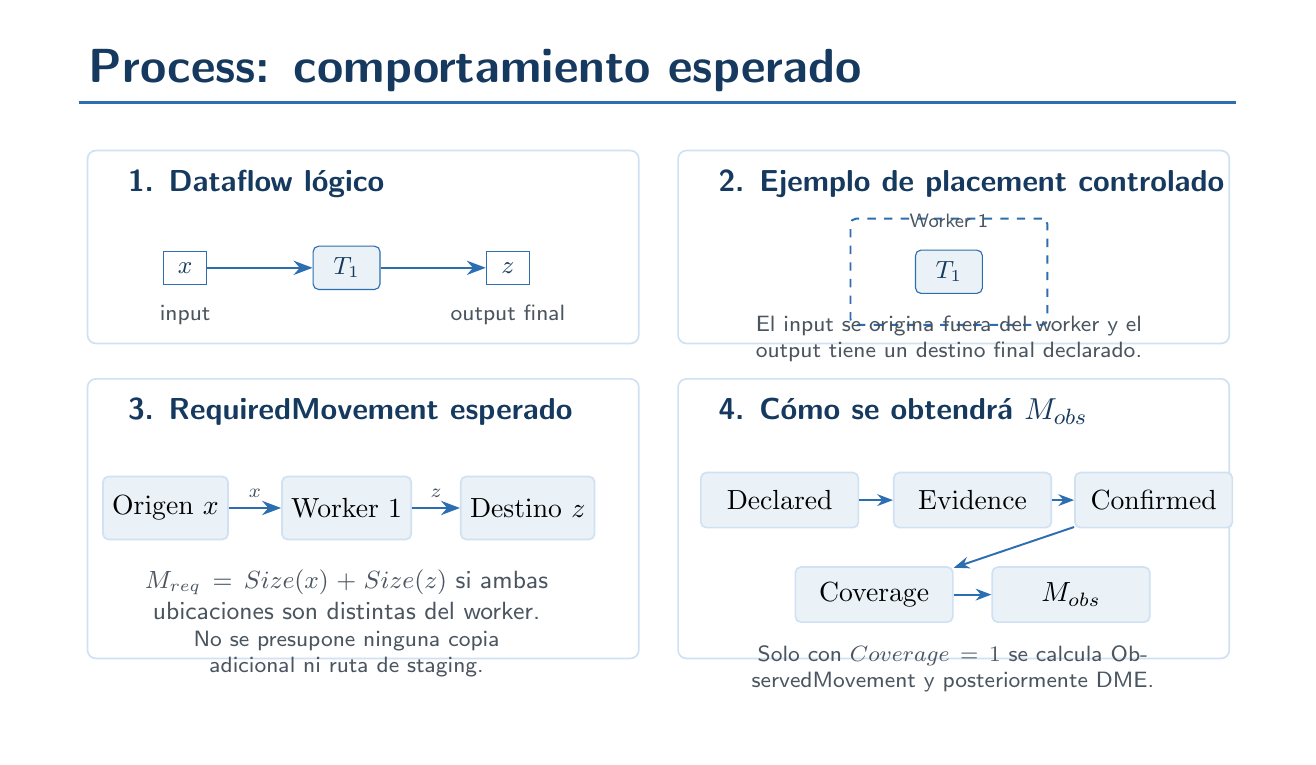
\begin{tikzpicture}[x=1cm,y=1cm]
\path[use as bounding box] (0,0) rectangle (16,9);
\node[title] at (0.65,8.45) {Process: comportamiento esperado};
\draw[blue,line width=1pt] (0.65,8.05)--(15.35,8.05);
\node[panel,minimum width=7cm,minimum height=2.45cm,anchor=north west] at (0.75,7.45) {};
\node[subtitle,anchor=west] at (1.15,7.02) {1. Dataflow lógico};
\node[file] (x) at (2.0,5.95) {$x$}; \node[task] (t1) at (4.05,5.95) {$T_1$}; \node[file] (z) at (6.1,5.95) {$z$};
\draw[arr] (x)--(t1); \draw[arr] (t1)--(z);
\node[small] at (2.0,5.35) {input}; \node[small] at (6.1,5.35) {output final};
\node[panel,minimum width=7cm,minimum height=2.45cm,anchor=north west] at (8.25,7.45) {};
\node[subtitle,anchor=west] at (8.65,7.02) {2. Ejemplo de placement controlado};
\node[worker,minimum width=2.5cm,minimum height=1.35cm] at (11.7,5.9) {};
\node[tinylabel] at (11.7,6.55) {Worker 1}; \node[task] at (11.7,5.9) {$T_1$};
\node[small,text width=5.7cm,align=center] at (11.7,5.05) {El input se origina fuera del worker y el output tiene un destino final declarado.};

\node[panel,minimum width=7cm,minimum height=3.55cm,anchor=north west] at (0.75,4.55) {};
\node[subtitle,anchor=west] at (1.15,4.12) {3. RequiredMovement esperado};
\node[box,minimum width=1.55cm,minimum height=0.8cm] (src) at (1.75,2.9) {Origen $x$};
\node[box,minimum width=1.55cm,minimum height=0.8cm] (w) at (4.05,2.9) {Worker 1};
\node[box,minimum width=1.55cm,minimum height=0.8cm] (dst) at (6.35,2.9) {Destino $z$};
\draw[arr] (src)-- node[above,tinylabel] {$x$} (w); \draw[arr] (w)-- node[above,tinylabel] {$z$} (dst);
\node[body,text width=5.9cm,align=center] at (4.05,1.8) {$M_{req}=Size(x)+Size(z)$ si ambas ubicaciones son distintas del worker.};
\node[small,text width=5.8cm,align=center] at (4.05,1.05) {No se presupone ninguna copia adicional ni ruta de staging.};

\node[panel,minimum width=7cm,minimum height=3.55cm,anchor=north west] at (8.25,4.55) {};
\node[subtitle,anchor=west] at (8.65,4.12) {4. Cómo se obtendrá $M_{obs}$};
\node[box,minimum width=2.0cm,minimum height=0.7cm] (d) at (9.55,3.0) {Declared};
\node[box,minimum width=2.0cm,minimum height=0.7cm] (e) at (12.0,3.0) {Evidence};
\node[box,minimum width=2.0cm,minimum height=0.7cm] (c) at (14.3,3.0) {Confirmed};
\draw[arrthin] (d)--(e); \draw[arrthin] (e)--(c);
\node[box,minimum width=2.0cm,minimum height=0.7cm] (cov) at (10.75,1.8) {Coverage};
\node[box,minimum width=2.0cm,minimum height=0.7cm] (obs) at (13.25,1.8) {$M_{obs}$};
\draw[arrthin] (c)--(cov); \draw[arrthin] (cov)--(obs);
\node[small,text width=5.7cm,align=center] at (11.75,0.85) {Solo con $Coverage=1$ se calcula ObservedMovement y posteriormente DME.};
\end{tikzpicture}
\end{document}
